%+----------------------------------------------------------------------------
%| SLIDES: Phd Thesis - Private Defence
%| Contents: - 10 Techincal Slides  
%|					 (extimated duration 3 minutes per slide )
%|			 - Backup Slides on technical points			
%| Author: Antonio miti
%| Place: Leuven, September 2019
%+----------------------------------------------------------------------------+


%- HandOut Flag -----------------------------------------------------------------------------------------
\newif\ifHandout
%	\Handouttrue  %uncomment for the printable version


%- D0cum3nt ----------------------------------------------------------------------------------------------
\ifHandout
	\documentclass[handout,10pt]{beamer}   
	\setbeameroption{show notes} %print notes   
\else
	\documentclass[10pt]{beamer}
\fi



%- Packages ----------------------------------------------------------------------------------------------
\usepackage{custom-style}
\usepackage{array}
\usepackage{pbox}

%--Beamer Style-----------------------------------------------------------------------------------------------
\usetheme{toninus}




%- T1tle P4g3 -------------------------------------------------------------------------------------------
\title{Homotopy comomentum maps in Multisymplectic Geometry} 
\subtitle{\href{https://set.kuleuven.be/phd/sap/prelim}{Preliminary Defence}}
\author[AMM]{\href{https://dmf.unicatt.it/miti/}{Antonio Michele Miti}}
\institute[UCSC and KU Leuven]{
  \begin{tabular}[h]{ccc}
      Università Cattolica del Sacro Cuore & $\qquad$ & KU Leuven \\
      Brescia, Italy & & Leuven, Belgium \\
      \href{https://dipartimenti.unicatt.it/dmf-home?rdeLocaleAttr=it}{\includegraphics[width=3.5cm]{./Logos/UnicattBS-logo}} & & 
      \href{https://wis.kuleuven.be/english}{\includegraphics[width=4cm]{./Logos/KULeuven_logo}}
  \end{tabular}      
}
\date[PrivateDefence_21] % (optional, should be abbreviation of conference name)
{	
	\href{https://set.kuleuven.be/phd/sap/dualjoint/oral}{International Doctoral Programme in Science } \\
	{\vskip 1ex}
	February 2, 2021
}





\newcommand{\thankyouslide}[0]{
	\ifHandout

	\else
	\addtocounter{framenumber}{-1}
	\begin{frame}{}
		\vfill
	  \centering 
	  {\Huge\color{red} 
	  \emph{Thank you for your attention!}}
		\vfill
		%
		\centering
		\begin{columns}
			\hfill
			\begin{column}{0.05\linewidth}
				\centering \includegraphics{beamericonarticle}
			\end{column}
			\begin{column}{0.8\linewidth}
				\centering
				\textbf{On some (multi)symplectic aspects of link invariants},
				\\
				\emph{AMM, Mauro Spera}, \href{https://arXiv.org/abs/1805.01696}{arxiv:1805.01696};\\
				(to appear in \emph{Journal of the Australian Mathematical Society})	
			\end{column}
			\begin{column}{0.05\linewidth}
				\centering \includegraphics{beamericonarticle}			
			\end{column}
			\hfill
		\end{columns}
		\vfill
		\begin{columns}
			\hfill
			\begin{column}{0.05\linewidth}
				\centering \includegraphics{beamericonarticle}
			\end{column}
			\begin{column}{0.8\linewidth}
				\centering
				\textbf{Multisymplectic actions of compact Lie groups on spheres},
				\\
				\emph{AMM, Leonid Ryvkin}, \href{https://arxiv.org/abs/1906.08790}{arXiv:1906.08790};
				\\
				(to appear in \emph{Journal of Symplectic Geometry})
			\end{column}
			\begin{column}{0.05\linewidth}
				\centering \includegraphics{beamericonarticle}			
			\end{column}
			\hfill
		\end{columns}		
		\vfill		
		\begin{columns}
			\hfill
			\begin{column}{0.05\linewidth}
				\centering \includegraphics{beamericonarticle}
			\end{column}
			\begin{column}{0.8\linewidth}
				\centering
		\textbf{Derivation of the HOMFLYPT knot polynomial via helicity and geometric quantization},
				\\
		\emph{AMM, Mauro Spera}, \href{https://arxiv.org/abs/1910.13400}{arXiv:1910.13400};\\
				(to appear in \emph{Bollettino dell'Unione Matematica Italiana})	
			\end{column}				
			\begin{column}{0.05\linewidth}
				\centering \includegraphics{beamericonarticle}			
			\end{column}
			\hfill
		\end{columns}
		\vfill
		\begin{columns}
			\hfill
			\begin{column}{0.05\linewidth}
				\centering \includegraphics{beamericonarticle}
			\end{column}
			\begin{column}{0.8\linewidth}
				\centering
				\textbf{Observables of multisymplectic manifolds and higher Courant algebroids},
				\\
				\emph{AMM, Marco Zambon}; % \href{https://arXiv.org/abs/1805.01696}{arxiv:1805.01696};\\
				(To appear soon on \emph{arxiv})	
			\end{column}
			\begin{column}{0.05\linewidth}
				\centering \includegraphics{beamericonarticle}			
			\end{column}
			\hfill
		\end{columns}
	\end{frame}
	\fi
}






%---------------------------------------------------------------------------------------------------------------------------------------------------
%- D0cum3nt ----------------------------------------------------------------------------------------------------------------------------------
\begin{document}
%-------------------------------------------------------------------------------------------------------------------------------------------------
\begin{frame}  % Alternative: \maketitle outside of frame
	\titlepage
	\ifHandout
		\tikz[overlay,remember picture]
		{
	    	%	\node at ($(current page.west)+(1.5,0)$) [rotate=90] {\Huge\textcolor{gray}{\today}};
	    	\node[        
	    		draw,
	    		shape border rotate=90,
			isosceles triangle,
			isosceles triangle apex angle=90,
			fill=yellow]
	        		at ($(current page.north east)-(1,1)$) [rotate=-45] {\textcolor{red}{Handout version}};
		}
	\fi
	\end{frame}
	\addtocounter{framenumber}{-1}
\note{
	%Abstract?
	\textbf{\underline{OUTLINE}}:
	\tableofcontents
}
%---------------------------------------------------------------------------------------------------------------------------------------------------
\outline


%-------------------------------------------------------------------------------------------------------------------------------------------------
\subsubsection{Introduction}
\begin{frame}[fragile]{Multisymplectic geometry in a nutshell}
	\begin{block}{Historical motivation}
		Mechanics: geometrical foundations of \textit{(first-order)} field theories.
	\end{block}
	\vfill	
	\begin{table}
		\only<2>{
		\begin{tabular}{|p{0.2\textwidth}|p{0.3\textwidth}|p{0.35\textwidth}|} 
            \hline
            \parbox[][20pt][c]{0.2\textwidth}{mechanics} & \multicolumn{2}{c|}{geometry} \\
            \hline
            \parbox[][20pt][c]{0.2\textwidth}{phase space} & symplectic manifold &  \\[.25em]
            \parbox[][20pt][c]{0.2\textwidth}{classical \\ observables} & Poisson algebra &  \\[.25em]
            \parbox[][20pt][c]{0.2\textwidth}{symmetries} &  group actions admitting comoment map &  
            \\
            \hline
  \multicolumn{1}{c}{}
            &  \multicolumn{1}{@{}c@{}}{$\underbrace{\hspace*{.3\textwidth}}_{\text{point-like particles systems}}$} 
            &  \multicolumn{1}{@{}c@{}}{}              \\
		\end{tabular}
		
		
		}
		\onslide<3->{
		\begin{tabular}{|p{0.2\textwidth}|p{0.3\textwidth}|p{0.35\textwidth}|} 
            \hline
            \parbox[][20pt][c]{0.2\textwidth}{mechanics} & \multicolumn{2}{c|}{geometry} \\
            \hline
            \parbox[][20pt][c]{0.2\textwidth}{phase space} & symplectic manifold & multisymplectic manifold \\[.25em]
            \parbox[][20pt][c]{0.2\textwidth}{classical \\ observables} & Poisson algebra & $L_\infty$-algebra \\[.25em]
            \parbox[][20pt][c]{0.2\textwidth}{symmetries} &  group actions admitting comoment map & group actions admitting 
			\tikz[baseline,remember picture]{\node[rounded corners,
                        fill=orange!10,draw=orange!30,anchor=base]            
            			(target) {homotopy comomentum map};
            }
            \\
            \hline
  \multicolumn{1}{c}{}
            &  \multicolumn{1}{@{}c@{}}{$\underbrace{\hspace*{.3\textwidth}}_{\text{point-like particles systems}}$} 
            &
            \multicolumn{1}{@{}c@{}}{$\underbrace{\hspace*{.3\textwidth}}_{\text{field-theoretic systems}}$} 
               \\
		\end{tabular}
		}
	\end{table}		
	\vfill
	\onslide<4->{
	
	\begin{block}{Scope of the thesis}
		\begin{itemize}
			\item[$\bullet$] Develop theory of 
				\tikz[baseline,remember picture]{\node[rounded corners,
                        fill=orange!10,draw=orange!30,anchor=base]            
            			(base) {homotopy comomentum maps};
            	}
            \item[$\bullet$] produce new meaningful examples.
		\end{itemize}
	\end{block}


                    \begin{tikzpicture}[overlay,remember picture]
                    \path[->]<4-> (base.north east) edge[bend right](target.south east);
                    \end{tikzpicture}
	}


\end{frame}
\note[itemize]{
	\item Historically, the interest in multisymplectic manifolds, has been motivated by the need for understanding the geometrical foundations of first-order classical field theories.
	The key point is that, just as one can associate a symplectic manifold to an ordinary classical mechanical system (e.g. a single
point-like particle constrained to some manifold), it is possible to associate a multisymplectic
manifold to any classical field system (e.g. a continuous medium like a filament or a fluid). See frame Extra-\ref{Frame:Ms-Field-Mechanics} 
	
	\item General ideas basic parallelisms with caveats
	\item caveat: points in multiphase spaces are not states
	\item the table hides the duality between geometric and algebraic approaches to the problem.
	\item 
}
%-------------------------------------------------------------------------------------------------------------------------------------------------



%-------------------------------------------------------------------------------------------------------------------------------------------------
\section{Background}
	\checkpoint
	\input{defence-background}
%-------------------------------------------------------------------------------------------------------------------------------------------------



%-------------------------------------------------------------------------------------------------------------------------------------------------
\section{Foreground}
%-------------------------------------------------------------------------------------------------------------------------------------------------

%-------------------------------------------------------------------------------------------------------------------------------------------------
	\subsection{Hydrodynamical homotopy moment map and Knots}
	\subcheckpoint	
	%+----------------------------------------------------------------------------+
%| SLIDES: 
%| Chapter: Results of the paper with M. Spera
%| Author: Antonio miti
%| Event: PHD  Defence
%+----------------------------------------------------------------------------+
%- HandOut Flag -----------------------------------------------------------------------------------------
\makeatletter
\@ifundefined{ifHandout}{%
  \expandafter\newif\csname ifHandout\endcsname
}{}
\makeatother

%- D0cum3nt ----------------------------------------------------------------------------------------------
\documentclass[beamer,10pt]{standalone}   
%\documentclass[beamer,10pt,handout]{standalone}  \Handouttrue  

\ifHandout
	\setbeameroption{show notes} %print notes   
\fi
	
%- Packages ----------------------------------------------------------------------------------------------
\usepackage{custom-style}

%--Beamer Style-----------------------------------------------------------------------------------------------
\usetheme{toninus}



%---------------------------------------------------------------------------------------------------------------------------------------------------
%- D0cum3nt ----------------------------------------------------------------------------------------------------------------------------------
\begin{document}
%------------------------------------------------------------------------------------------------


\begin{frame}{Applications to hydrodynamics and knot theory}\label{frame:hydro1}
	\begin{columns}[T] % align columns
	\begin{column}{.4\textwidth}
		\vspace{.5em}
		\centering
			\includegraphics[width=\linewidth]{Pictures/Figure_continuum}
	\end{column}
	%
	\hfill
	%
	\begin{column}{.6\textwidth}
		\scalebox{.8}{%
			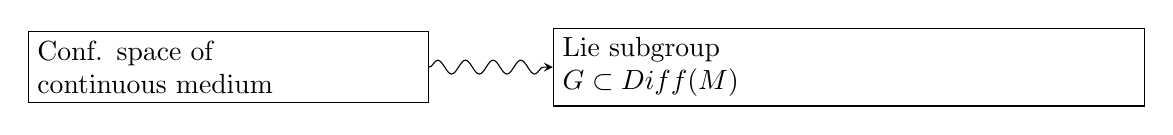
\begin{tikzpicture}[
				node distance=0.65\linewidth,
				]
				\node [text width=0.4\linewidth,rectangle,draw] (lhs) {Conf. space of\\ continuous medium};
				\node [text width=0.6\linewidth, rectangle,draw,right of=lhs] (rhs) {Lie subgroup \\$G \subset Diff(M)$};
				\draw[-stealth,decorate,decoration={snake}] (lhs) -- (rhs);
			\end{tikzpicture}
		}		
		Examples:
		\scalebox{.8}{%		
		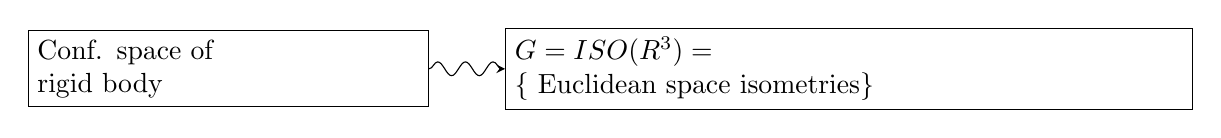
\begin{tikzpicture}[
			node distance=0.65\linewidth,
			]
			\node [text width=0.4\linewidth,rectangle,draw] (lhs) {Conf. space of\\ rigid body};
			\node [text width=0.7\linewidth,rectangle,draw,right of=lhs] (rhs) {$G=ISO(\mathbb{R}^3)=$\\ $\{$
				Euclidean space isometries$\}$};
			\draw[-stealth,decorate,decoration={snake}] (lhs) -- (rhs);
		\end{tikzpicture}
		}
		\scalebox{.8}{%
		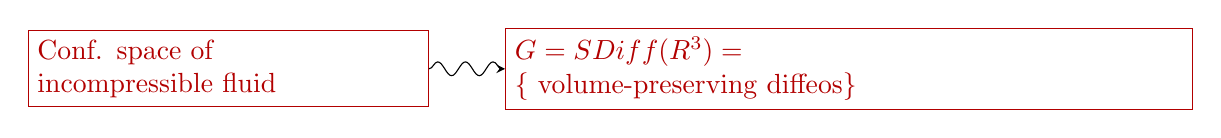
\begin{tikzpicture}[
			node distance=0.65\linewidth,
			]
			\node [text width=0.4\linewidth,red!70!black,rectangle,draw] (lhs) {Conf. space of\\ incompressible fluid};
			\node [text width=0.7\linewidth,red!70!black,rectangle,draw,right of=lhs] (rhs) {$G= SDiff(\mathbb{R}^3)=$\\ $\{$
				volume-preserving diffeos$\}$};
			\draw[-stealth,decorate,decoration={snake}] (lhs) -- (rhs);
		\end{tikzpicture}
		}
	\end{column}%
	\end{columns}
	\pause
	\vfill
	We consider the following setting:
	
	\begin{itemize}%[<+->]
		\item[$\bullet$]2-plectic manifold: 
		\vspace{-1em} 
			$$M=(\mathbb{R}^3,\nu = dx\wedge dy\wedge dz)$$
			\vspace{-.8em}\pause
		\item[$\bullet$]$\infty$-dim. Lie algebra (\emph{ideal fluid velocities}): \vspace{-1em}
			$$\mathfrak{g}:= sdiff_0(\mathbb{R}^3) = \left\lbrace  X \in \mathfrak{X}(\mathbb{R}^3) ~\left\vert~ 
		  		\substack{ div X = 0, \\ \textrm{\emph{ rapidly vanishing at }}\infty} \right\rbrace \right.$$
		  	\vspace{.2em}\pause
		\item[$\bullet$] Multisymplectic Lie algebra action:
			\vspace{-1em} 
			$$\mathfrak{g}= sdiff_0 \hookrightarrow  \mathfrak{X}(\mathbb{R}^3)$$
\end{itemize}		
	\pause
	\vfill
	\begin{center}
	\tcbox[enhanced,frame hidden,borderline={0.5pt}{0pt}{red,dashed}]{	
		\alert{
		\faQuestionCircle \qquad
			{Does $sdiff_0 \circlearrowleft (\mathbb{R}^3,\nu = dx\wedge dy\wedge dz)$ admit an HCMM?}	
		\qquad \faQuestionCircle		
		}
	}
	\end{center}

\end{frame}
\note[itemize]{
	\item We are working in the setting of \emph{geometric continuum mechanics} .\\
		Recall that the configuration space of a continuum object is encoded via diffeomorphisms. In the case of an incompressible fluid is encoded via volume-preserving diffeomorphisms.
	\item (Configution space is the set of spatial displacement of a mechanical systems. These are different from the \emph{physical states}.
	\item Such manifolds are infinite dimensional. Particular caution has to be taken in defining the smooth structure in this case.
	\item However, what really matters in the construction of a moment map is the infinitesimal action, i.e. the Lie algebra. In our case, the infinitesimal action to be considered is via divergence-free vector fields.
	\item (Notation): In the following M will be the 3 dimensional Euclidean Space.
	\item The simple but crucial observation is that the standard volume form on the euclidean space is a multisymplectic form.


}



%---------------------------------------------------------------------------------------------------------------------------------------------------
\begin{frame}{A Hydrodynamical HCMM}\label{frame:hydro2}
	\begin{columns}
		\begin{column}[c]{.5\linewidth}
		  	\begin{itemize}
		  		\item The observables are  $$L= \Omega^1_{\textrm{ham}}(\mathbb{R}^3)\oplus\Omega^0(\mathbb{R}^3)$$
		  		\item \hyperlink{frame:hydromomap-details}{HCMM consists of a pair of functions}:
					\begin{align*}
						f_1 &\colon \mathfrak{g} \rightarrow \Omega^1_{\textrm{ham}}(\mathbb{R}^3) \\
						f_2 &\colon \mathfrak{g}\wedge\mathfrak{g} \rightarrow C^\infty(\mathbb{R}^3)
					\end{align*}	
		  	\end{itemize}
		\end{column}	
	  	\hfill  	
		\begin{column}[c]{.5\linewidth}
  		\includestandalone[width=\textwidth]{Pictures/Figure_Euclid_Trigger}
 	 	\end{column}
 	 \end{columns}


	\pause
\tcbset{colback=white,
	colbacktitle=white,
	colframe=blue!70!black,
	boxrule=1pt,
	colupper=blue!70!black,
	arc=15pt,
	}
	\begin{tcolorbox}[sidebyside,righthand width=.75\linewidth]
		Thm: \cite{Miti2018}
		\tcblower
		\vspace{-1.5em}
		\begin{columns}
		\begin{column}{.6\linewidth}	
		\begin{align*}
		f_1 &= \flat \circ \text{curl}^{-1} 
		%~:~ \mathfrak{g} \to \Omega^{1}_{Ham}(\mathbb{R}^3)
		%\qquad \text{\small ("Biot-Savart law")}
		%\tag{\small"Biot-Savart law"}
		\\
		f_2 &= \Delta^{-1} \circ \delta \circ (f_1 \circ \partial_{CE} +\iota(\cdot)\omega) 
		%~:~ \wedge^2\mathfrak{g} \to C^{\infty}(\mathbb{R}^3)
		%\tag{\small"Coulomb law"}
		\end{align*}		
		\end{column}	
		\begin{column}{.5\linewidth}
			\begin{center}
				\tikz[baseline,remember picture]{\node[rounded corners,
                        fill=orange!5,draw=orange!30,anchor=base]            
            			(base) [rotate=-0,text width=3cm,align=left]{
            				\hyperlink{frame:RiemannianGeneralization}{
            					\footnotesize{
            					Riemannian structure\\\quad plays a crucial role
							}            				
            				}
            			};
            	}		
			\end{center}					
		\end{column}			
		\end{columns}	
	\end{tcolorbox}
	\pause
	\vfill
	\hyperlink{frame:hydro-reinterpretation}{Getting back to hydrodynamics}:
	\begin{tcolorbox}[sidebyside,righthand width=.75\linewidth]
		Thm: \cite{Miti2018}
		\tcblower
		HCMM for $G\circlearrowright(\mathbb{R}^3,\nu)$ induces an ordinary co-mo.map for $G\circlearrowright (LS,\nu^{\ell})$ via \emph{trasgression.}
		\\[.5em]
		\hyperlink{frame:HydroHCMM-reinterpretation}{\alert{\small\emph{(Arnol'd-Marsden-Weinstein hydrodynamical co-momentum map)}}}
		\vfill			
	\end{tcolorbox}


\end{frame}
\note[itemize]{
	\item relation with knot theory: looking at the knot as a fluid configuration with singular vorticity along a knotted tube,
	\item subalgebra of the infinitesimal action of $SDiff(\mathbb{R}^3)$
	\item observe how elements from Riemannian geometry and hodge theory appear in the construction
		\begin{itemize}
			\item $\delta$ codifferential
			\item $\Delta$ Laplacian
			\item $\flat$ $\sharp$  musical isomorphisms
		\end{itemize}

	\item
	Applications:
	\begin{itemize}[<+->]%[<alert@+>]
		\item[\CheckedBox]  Hydrodynamics interpretation: Rasetti-Regge currents as "momenta".
		% is exhibited upon resorting to the Euler equation for perfect fluids.
		\item[\CheckedBox]  Knot theory: reinterpretation of the (Massey) higher order linking numbers in terms of conserved quantities.
		\item[\CheckedBox]  Semiclassical interpretation of the HOMFLYPT polynomial.
	\end{itemize}

	\item other results of the paper: 	
	\begin{itemize}
		\item[\CheckedBox]  Explicit construction of an HCMM for $SDiff_0 \circlearrowright (\mathbb{R}^3,\nu)$ (and generalization to Riemannian homological spheres);
		\item[\CheckedBox]  Hydrodynamics interpretation: proved that this HCMM trasgresses to the standard hydrodynamical co-momentum map of  Arnol'd, Marsden and Weinstein and others; (we recover a quantitity already in use in mechanics)
		% is exhibited upon resorting to the Euler equation for perfect fluids.
		\item[\CheckedBox]  Application to knot theory: reinterpretation of the (Massey) higher order linking numbers in terms of conserved quantities and determined the knot theoretic analogues of first integrals in involution.



	\end{itemize}
	
}
%---------------------------------------------------------------------------------------------------------------------------------------------------



%---------------------------------------------------------------------------------------------------------------------------------------------------
  \begin{frame}{Knot differential forms as observables}\label{frame:hydro3}
	IDEA: Vortex theory approach to knots:
	\begin{itemize}
		\item[\xmark] knots as embeddings $S^1\hookrightarrow \mathbb{R}^3$.
		\item[\cmark] knots as ideal fluid configurations with vorticity concentrated on closed curves
	\end{itemize}
	\pause
	%
	\vfill
  	\begin{columns}
		\begin{column}[c]{.7\linewidth}	
				Let $ L = \cup_{i=1}^n L_i$ be an oriented link in ${\mathbb R}^3$ 
				\\(components $L_i$, $i=1,\dots,n$ required to be  {\it trivial} knots)	
		\end{column}
		\begin{column}[c]{.25\linewidth}
			\centering{
			\includegraphics[width=0.75\linewidth]{./Pictures/Whiteheadlink}
			}
		\end{column}
  	\end{columns}
	%
	\pause
  	\begin{columns}
		\begin{column}[t]{.5\linewidth}	
			\begin{defblock}[Vorticity 2-form]
				$$
				\omega_{L} := \sum_{i=1}^n \omega_{L_i}, \qquad d\omega_L = 0
				$$
				($\omega_{ L_i}$ = \hyperlink{frame:poinduals}{Poincar\'e dual} associated to $L_i$)
			\end{defblock}
		\end{column}
		\begin{column}[t]{.5\linewidth}	
			\begin{defblock}[Velocity 1-form]
				\vspace{-.75em}
				$$
 					v_{ L} = \sum_{i=1}^n v_{L_i}, \qquad \qquad  dv_{L} = \omega_{ L}
				$$
				($v_{L_i} := \omega_{{\mathfrak a}_i}$ = \hyperlink{frame:poinduals}{Poincar\'e dual}  of a disc ${\mathfrak a}_i$ 
				bounded by 	$L_i$ \footnotesize{(Seifert surface)}) 
			\end{defblock}						
		\end{column}
  	\end{columns}
	%
	\pause
	%
	\tcbset{colback=white,
	colbacktitle=white,
	colframe=blue!70!black,
	boxrule=1pt,
	colupper=blue!70!black,
	arc=15pt,
	}
	\begin{tcolorbox}[sidebyside,righthand width=.7\linewidth]
		Thm: \cite{Miti2018}
		\tcblower
		$v_{L}$ is a {\it Hamiltonian 1-form}
		\\[.5em]
		\pause
		\hyperlink{frame:highorderlinking}{\footnotesize{(the same applies to every \emph{"higher velocity $1-form$})}}.
	\end{tcolorbox}	
	 

  
  \end{frame}
  \note[itemize]{
  	\item $G~=~SDiff_0(\mathbb{R}^3)$	(volume-preserving diffeomorphisms) encompasses ambient isotopies of knotted links (interpreted as singular vortices) and Euler evolution
	\item "instead as considering the knot we focus on its complementary"
	\item the context allows to understand certain knot theoretic quantities as hamiltonian forms
	\item $\omega_{ L_i}$ denote the Poincar\'e (or Thom) dual (class) associated to $L_i$: they are 2-forms localized in a 
 cross-section of a  suitable tubular neighbourhood $T_i$ around $L_i$ - with total fibre integral equal to one, or, as currents, 2-forms which are $\delta$-like on $L_i$
 
	\item $v_{L_i} := \omega_{{\mathfrak a}_i}$ is the Poincar\'e dual (class) of a disc ${\mathfrak a}_i$ bounding
$L_i$ (a Seifert surface for the trivial knot $L_i$). Precisely:
$$
\partial {\mathfrak a}_i = L_i, \qquad \qquad dv_{L_i} = d\omega_{{\mathfrak a}_i} = \omega_{L_i} = \omega_{\partial {\mathfrak a}_i},
$$
	\item
		Velocity 1-forms $v_i$ correspond (upon approximation of the associated Euler equation) to the so-called LIA (Linear Induction Approximation) or  {\it binormal evolution}
		of the ``vortex ring" $L_i$ (``orthogonal" to the discs ${\mathfrak a}_i$.
		
	\item Everything is up to choices of tubular neighbourhoods, Seifert surface and specific Poincar\'e dual.	
	
}
%------------------------------------------------------------------------------------------------





%----------------------------------------------------------------------------------------------------------------------------------
\end{document}
%----------------------------------------------------------------------------------------------------------------------------------

%-------------------------------------------------------------------------------------------------------------------------------------------------
%-------------------------------------------------------------------------------------------------------------------------------------------------
	\subsection{Multisymplectic compact group actions on spheres}
	\subcheckpoint	
	\input{defence-spheres}
%-------------------------------------------------------------------------------------------------------------------------------------------------
%-------------------------------------------------------------------------------------------------------------------------------------------------
	\subsection{Gauge transformations, higher Courant algebroids and HCMM}
	\subcheckpoint	
	%+----------------------------------------------------------------------------+
%| SLIDES: 
%| Chapter: Results of the paper with M. Zambon
%| Author: Antonio miti
%| Event: PHD preliminary Defence
%+----------------------------------------------------------------------------+

%- HandOut Flag -----------------------------------------------------------------------------------------
\newif\ifHandout

%- D0cum3nt ----------------------------------------------------------------------------------------------
\documentclass[beamer,10pt]{standalone}   
%\documentclass[beamer,10pt,handout]{standalone}  \Handouttrue  

%- HandOut Flag -----------------------------------------------------------------------------------------
\ifHandout
	\setbeameroption{show notes} %print notes   
\fi

	
%- Packages ----------------------------------------------------------------------------------------------
\usepackage{custom-style}

%--Beamer Style-----------------------------------------------------------------------------------------------
\usetheme{toninus}






%---------------------------------------------------------------------------------------------------------------------------------------------------
%- D0cum3nt ----------------------------------------------------------------------------------------------------------------------------------
\begin{document}
%------------------------------------------------------------------------------------------------


%TITOLO DA AGGIORNARE
%-------------------------------------------------------------------------------------------------------------------------------------------------
%\subsection{Commutative diagram with gauge transformations and HCMM}
%-------------------------------------------------------------------------------------------------------------------------------------------------


%-------------------------------------------------------------------------------------------------------------------------------------------------
\begin{frame}[fragile]{Compatibility between gauge transformations and comoment maps}
	%
	Consider $(M,\omega)$ \alert{symplectic mfd.}
	\only<5-11>{ and \alert{\underline{prequantizable}} ($S^1$-bundle $P$, connection $\theta$)}
	%
	\begin{center}
			\includestandalone[width=.8\textwidth]{Pictures/Frame_BigDiagram_symplectic}
	\end{center}
	%
	\vspace{-2em}
	\begin{minipage}[t][1.7cm][t]{\textwidth}
	\begin{itemize}
		\only<1-4>{
			\item<2-> Given a Symp. mfd. $(M,\omega)$ there is a naturally associated Poisson algebra ...
			\item<3-> .\alert<+>{... and also a Lie Algebroid}.
			\item<4-> A Lie algebroid is a "controlled" $\infty$-dimensional Lie algebra;
		}
		\only<5-6>{
			\item<5-> Prequantization Bundle $S^1\hookrightarrow P \to M$ with connection $\theta$,
			\item<5-> "infinitesimal quantomorphisms" $Q(P,\theta):=\lbrace Y \in \mathfrak{X}(P)~|~ \mathcal{L}_Y \theta =0 \}$.
		}
		\only<7-11>{
		\item<7-> Consider a deformed structure $\tilde{\omega}= \omega + d B$ with $B\in C^\infty(M)$;
		\item<9-> There is a natural isomorphism in the Lie Alg.oids category,
		\item<11-> Considering $\mathfrak{g}\circlearrowleft M$ preserving $\omega$ and $\tilde{\omega}$ ...
		}
		\item<12-> Neglect the prequantization...
		\vspace{-1em} 
			\begin{displaymath}
				\begin{tikzcd}
					\Psi~:&[-1em] C^{\infty}(M)_\omega \ar[r,"\Psi"]& \Gamma(TM\oplus \mathbb{R})_\omega
					\\[-2em]
					& f \ar[r,mapsto] & \binom{\mathscr{v}_f}{f}
				\end{tikzcd}
			\end{displaymath}
	\end{itemize}
	\end{minipage}
	\vfill
	\tcbset{colback=white,
	colbacktitle=white,
	colframe=red!70!black,
	boxrule=1pt,
	colupper=red!70!black,
	arc=15pt,
	}
	\begin{minipage}[t][1.7cm][t]{\textwidth}
	\only<6>{ 
		\begin{tcolorbox}[enhanced,frame hidden,borderline={0.5pt}{0pt}{blue}]
			\color{blue}{
			The left square and right triangles commutes!
			}
		\end{tcolorbox}
	}
	\only<11>{
		\begin{tcolorbox}[enhanced,frame hidden,borderline={0.5pt}{0pt}{blue}]
			\color{blue}{
			The left square and right triangle commute!
			}
		\end{tcolorbox}
	}
	\only<12>{
		\vspace{-.75em}
		\begin{tcolorbox}[enhanced,frame hidden,borderline={0.5pt}{0pt}{blue}]
			\color{blue}{
			The central pentagon commutes!
			}
		\end{tcolorbox}
	\vfill
		\vspace{-.75em}
		\begin{center}
		\tcbox[enhanced,frame hidden,borderline={0.5pt}{0pt}{red,dashed}]{	
			\alert{
			\faQuestionCircle \qquad
				{What happens in the higher (n-plectic) case?}
			\qquad \faQuestionCircle		
			}
		}
		\end{center}
	}
	\end{minipage}
	%
\end{frame}
\note[itemize]{
	\item The horizontal embedding is  $f \mapsto (v_f,f)$;
	\item Vertical maps are also known as \emph{Gauge transformations}
	\item upshot: 
	\begin{enumerate}
		\item 
	\end{enumerate}
}
%-------------------------------------------------------------------------------------------------------------------------------------------------


%-------------------------------------------------------------------------------------------------------------------------------------------------
\begin{frame}[fragile]{Embedding observables $L_\infty$-algebra into Vinogradov $L_\infty$-algebra}
	Consider now $\omega$ \alert{$n$-plectic}
	\vfill
	\begin{center}
		\includestandalone[width=.8\textwidth]{Pictures/Frame_Embedding_Diagram_k-plectic_V1}
	\end{center}
	\vfill
	\only<1-3>{
	\begin{itemize}
		\item<2-> Higher analogue of the Courant algebroid $\rightsquigarrow$ \alert{\emph{Vinogradov algebroid}}
			\begin{displaymath}
			E^n = \left(TM\oplus\bigwedge^{k-1}T^\ast M \right)
			\end{displaymath}
		\item<3->  Vin. alg.oids are $NQ$-manifolds ($L_\infty$-algebroids).
		\\ Associated $L_\infty$-algebra on the graded vector space
		\begin{displaymath}\label{eq:VSpace}
			{\mathcal{V}^k} =
			\begin{cases}
				\mathfrak{X}(M)\oplus \Omega^{n-1}(M)  &\quad k=0,\\
				\Omega^{n-1+k}(M) &\quad -n+1 \leq k < 0.
			\end{cases}
		\end{displaymath}
	\end{itemize}
	}


	\only<4->{
	\begin{thmblock}[Embedding of $L_\infty$-algebras  $\Psi:L_\infty(M,\omega)\hookrightarrow L_{\infty}(E^n,\omega)$\quad \cite{Miti2021}.]
	\begin{itemize}[leftmargin=0pt]
		\item[$\cdot$]<4-> 
			consider the graded vector subspace $\mathcal{A}$
			\begin{displaymath}
			\mathclap{
			{\mathcal{A}^k} =
			\begin{cases}
		\left.\left\lbrace
		\binom{X}{\alpha}\in \mathfrak{X}(M)\oplus \Omega^{n-1}(M)
		~ \right\vert ~
		\iota_X \omega = -d \alpha\right\rbrace
&\quad k=0,\\
				\Omega^{n-1+k}(M) &\quad -n+1 \leq k < 0.
			\end{cases}			
			}
			\end{displaymath}						
		\item[$\cdot$]<5-> 
			restrict the two $L_\infty$-structures to $\pi$ and $\mu$ on $\mathcal{A}$
		\item[$\cdot$]<6->

			$L_\infty(M,\omega) \cong 
				(\mathcal{A},\pi) \color{blue}\cong\color{black}
				(\mathcal{A},\mu) \hookrightarrow
				L_\infty(E^n,\omega)$
	\end{itemize}
	\end{thmblock}
	}
	\only<6->{
		\tikz[overlay,remember picture]
		{
			\node[rounded corners,
                 fill=orange!1,draw=orange!30,anchor=base]            
            	 (base) at ($(current page.east)-(2.25,4)$) [rotate=-0,text width=3cm,align=center] { \footnotesize{\color{red}{
            	 Complete proof\\
            	 \faWarning ~ up to $n\geq 4$! ~ \faWarning 
            	 }}};
		}			
	}

		

\end{frame}
\note{}
%-------------------------------------------------------------------------------------------------------------------------------------------------


%-------------------------------------------------------------------------------------------------------------------------------------------------
\begin{frame}{Compatibility with Gauge transformations}
	Consider now $\omega$ \alert{n-plectic} \quad and \alert{$\tilde{\omega}=\omega + d B$}:
	\vfill
	%
	\begin{center}
		\includestandalone[width=.8\textwidth]{Pictures/Frame_Gauge_Diagram_k-plectic}
	\end{center}	
	%
	\vfill
	%
	

	\begin{itemize}
	\only<1-3>{
		\item<2-> Vinogradov alg.oids w.r.t cohomologous twisting closed forms are isomorphic.
		\item<3-> Induced isomorphism at the level of $L_\infty$-algebras
	}
	\only<4->{
		\item<4-> Consider a Lie algebra action $\mathfrak{g}\to \mathfrak{X}(M)$ admitting HCMM w.r.t $\omega$ and $\tilde{\omega}$
	}
	\end{itemize}

	\vfill
	\tcbset{colback=white,
		colbacktitle=white,
		colframe=blue!70!black,
		boxrule=1pt,
		colupper=blue!70!black,
		arc=15pt,
		}
	\onslide<5->{
	\begin{tcolorbox}[sidebyside,righthand width=.75\linewidth]
		Thm: \cite{Miti2021}
		\tcblower
		\color{blue}
The central square commutes. 
			\\\emph{(On the nose, not "up to homotopies")}.
	\end{tcolorbox}	
		\tikz[overlay,remember picture]
		{
			\node[rounded corners,
                 fill=orange!1,draw=orange!30,anchor=base]            
            	 (base) at ($(current page.east)-(1.75,4)$) [rotate=-0,text width=3cm,align=center] { \footnotesize{\color{red}{
            	 Complete proof\\
            	 \faWarning ~ up to $n\geq 4$! ~ \faWarning 
            	 }}};
		}		
	
	
	}
	

\end{frame}
\note[itemize]{
	\item Our results can be seen as a tiny step toward  undestanding the analogue of prequantization in the setting of multisymplectic geometry (hence field theory).
}
%-------------------------------------------------------------------------------------------------------------------------------------------------




%----------------------------------------------------------------------------------------------------------------------------------
\end{document}
%----------------------------------------------------------------------------------------------------------------------------------





%-------------------------------------------------------------------------------------------------------------------------------------------------



\thankyouslide

%------------------------------------------------------------------------------------------------

%------------------------------------------------------------------------------------------------




%------------------------------------------------------------------------------------------------
% APPENDIX
%------------------------------------------------------------------------------------------------
\appendix
%-------------------------------------------------------------------------------------------------------------------------------------------------
\section{Complementary Material}
	\input{defence-complementary-material}
	%+----------------------------------------------------------------------------+
%| SLIDES: 
%| Chapter: Bibliography and Figures credit
%| Author: Antonio miti
%| Event: Phd Colloquium - What is ... Geometric mechanics?
%+----------------------------------------------------------------------------+

%- HandOut Flag -----------------------------------------------------------------------------------------
\makeatletter
\@ifundefined{ifHandout}{%
  \expandafter\newif\csname ifHandout\endcsname
}{}
\makeatother

%- D0cum3nt ----------------------------------------------------------------------------------------------
\documentclass[beamer,10pt]{standalone}   
%\documentclass[beamer,10pt,handout]{standalone}  \Handouttrue  

\ifHandout
	\setbeameroption{show notes} %print notes   
\fi

	
%- Packages ----------------------------------------------------------------------------------------------
\usepackage{custom-style}

%--Beamer Style-----------------------------------------------------------------------------------------------
\usetheme{toninus}








%---------------------------------------------------------------------------------------------------------------------------------------------------
%- D0cum3nt ----------------------------------------------------------------------------------------------------------------------------------
\begin{document}
%------------------------------------------------------------------------------------------------


\subsection{References}

%------------------------------------------------------------------------------------------------
% https://en.wikibooks.org/wiki/LaTeX/Bibliographies_with_biblatex_and_biber
\begin{frame}[t,allowframebreaks]{Extended Bibliography}
	%\nocite{*}
	\bibliographystyle{alpha}
	\bibliography{bibfile}
\end{frame}
%------------------------------------------------------------------------------------------------



%------------------------------------------------------------------------------------------------
\begin{frame}[t]{Other aknowledgements}
	\begin{itemize}
		\item Picture - Pendulum 13
			\url{https://andrewjobling.com.au/home-1/everything-okay-becasue-pendulum-swings/}
		\item Picture - Pendulum Phase Space
			\url{https://iopscience.iop.org/article/10.1088/0143-0807/33/2/231}
				\item Picture - Continuum deformation
			\url{https://commons.wikimedia.org/wiki/File:Displacement_of_a_continuum.svg}
		\item Animation - Reidmester moves
			\url{http://realworldmath.tumblr.com/post/57577812688/what-the-hell-is-knot-theory-knot-theory-is-one}
		\item Animation - Bubble rings
			\url{https://www.facebook.com/Nassim.Haramein.official/videos/596203997519126/}
		\item Picture - Whithead link 
			\url{https://en.wikipedia.org/wiki/Whitehead_link}
		\item Picture - Gauss linking number 
			\url{https://www.maths.ed.ac.uk/~v1ranick/papers/ricca.pdf}
		\item Picture - Borromean Rings
			\url{https://en.wikipedia.org/wiki/Borromean_rings}	
	\end{itemize}
\end{frame}
\note[itemize]{
	\item
}
%------------------------------------------------------------------------------------------------



%------------------------------------------------------------------------------------------------
\end{document}
%------------------------------------------------------------------------------------------------










%------------------------------------------------------------------------------------------------
\end{document}

